\documentclass[11pt]{article}

\usepackage[a4paper,margin=1in]{geometry}
\usepackage{amsmath,amssymb}
\usepackage{hyperref}
\hypersetup{
    colorlinks,
    citecolor=blue,
    filecolor=black,
    linkcolor=blue,
    urlcolor=blue
}
\usepackage{graphicx}
\usepackage{tikz}
\usetikzlibrary{arrows.meta}



\title{\textbf{The Jug Problem}}
\date{}
\begin{document}
\maketitle

\begin{center}
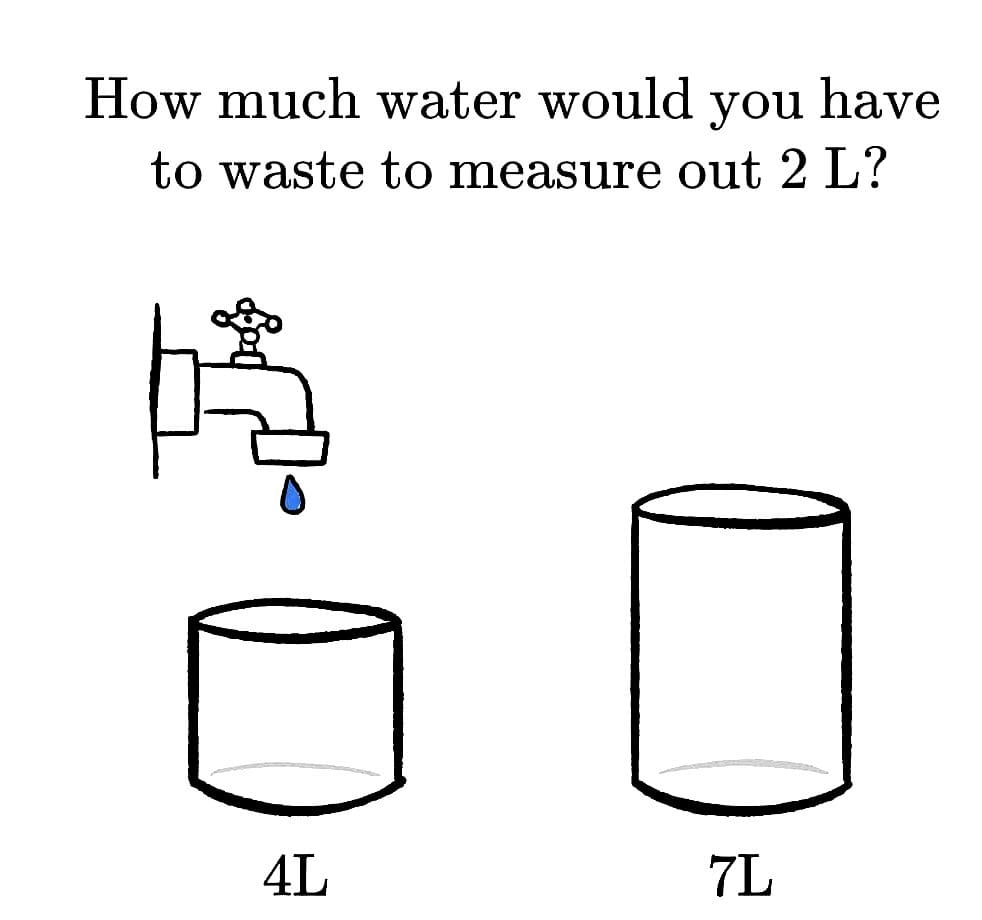
\includegraphics[width=2.5in]{jug.jpg}
\end{center}


\subsection*{Allowed Moves}

We represent a state of the system by an ordered pair
\[
(x,y),\qquad 0 \le x \le 4,\; 0 \le y \le 7,
\]
where $x$ is the amount of water in the 4-litre jug and $y$ is the amount
in the 7-litre jug.
The following six operations are allowed.

\begin{enumerate}
    \item \textbf{Fill the 4-litre jug from the tap}
    \[
    (x,y)\longrightarrow (4,y)
    \qquad\text{if } x<4.
    \]

    \item \textbf{Fill the 7-litre jug from the tap}
    \[
    (x,y)\longrightarrow (x,7)
    \qquad\text{if } y<7.
    \]

    \item \textbf{Empty the 4-litre jug into the drain}
    \[
    (x,y)\longrightarrow (0,y)
    \qquad\text{if } x>0.
    \]

    \item \textbf{Empty the 7-litre jug into the drain}
    \[
    (x,y)\longrightarrow (x,0)
    \qquad\text{if } y>0.
    \]

    \item \textbf{Pour from the 4-litre jug into the 7-litre jug}
    \[
    (x,y)\longrightarrow (x-t,\; y+t),
    \qquad
    t=\min\{x,\; 7-y\}.
    \]

    \item \textbf{Pour from the 7-litre jug into the 4-litre jug}
    \[
    (x,y)\longrightarrow (x+t,\; y-t),
    \qquad
    t=\min\{y,\; 4-x\}.
    \]
\end{enumerate}

Moves 3 and 4 are {\bf wastes} with costs $x$ and $y$ respectively. The other transitions in the graph (where the states are the nodes) have zero cost.

\subsection*{Invariant condition}
The only reachable states are ($x$ is 0 or 4) OR ($y$ is 0 or 7). See the following two figures.

%\begin{tikzpicture}[grow=down, level distance=10mm, sibling distance=20mm,
%                    every node/.style={circle,draw,inner sep=1pt}]
%\node{$(0,0)$}
% child {%
%   node{$(0,7)$}
%   child {%
%     node{$(4,3)$}
%     child {%
%       node{$(0,3)$}
%       child {%
%         node{$(3,0)$}
%         child {%
%           node{$(3,7)$}
%           child {%
%             node{$(4,6)$}
%             child {%
%               node{$(0,6)$}
%               child {%
%                 node{$(4,2)$}
%                 child {%
%                   node{$(0,2)$}
%                   child {%
%                     node{$(2,0)$}
%                   }
%                 }
%               }
%             }
%           }
%         }
%       }
%     }
%   }
%   child {%
%     node{$(4,7)$}
%   }
% }
% child {%
%   node{$(4,0)$}
%   child {%
%     node{$(0,4)$}
%     child {%
%       node{$(4,4)$}
%       child {%
%         node{$(1,7)$}
%         child {%
%           node{$(1,0)$}
%           child {%
%             node{$(0,1)$}
%             child {%
%               node{$(4,1)$}
%               child {%
%                 node{$(0,5)$}
%                 child {%
%                   node{$(4,5)$}
%                   child {%
%                     node{$(2,7)$}
%                   }
%                 }
%               }
%             }
%           }
%         }
%       }
%     }
%   }
% };
%\end{tikzpicture}

\vspace{0.5in}

\begin{figure}[ht]
\begin{center}
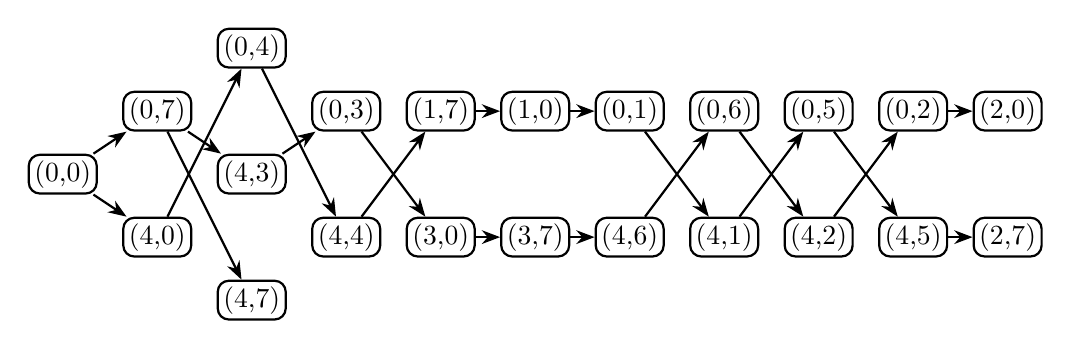
\begin{tikzpicture}[x=0.4cm,y=0.8cm,
  every node/.style={draw,rectangle,rounded corners,inner sep=2pt},
  >=Stealth, thick]

% nodes, grouped by BFS level (x = level)
\node (0_0) at (0,0)   {(0,0)};

\node (0_7) at (3,1)   {(0,7)};
\node (4_0) at (3,-1)  {(4,0)};

\node (0_4) at (6,2)   {(0,4)};
\node (4_3) at (6,0)   {(4,3)};
\node (4_7) at (6,-2)  {(4,7)};

\node (0_3) at (9,1)   {(0,3)};
\node (4_4) at (9,-1)  {(4,4)};

\node (1_7) at (12,1)  {(1,7)};
\node (3_0) at (12,-1) {(3,0)};

\node (1_0) at (15,1)  {(1,0)};
\node (3_7) at (15,-1) {(3,7)};

\node (0_1) at (18,1)  {(0,1)};
\node (4_6) at (18,-1) {(4,6)};

\node (0_6) at (21,1)  {(0,6)};
\node (4_1) at (21,-1) {(4,1)};

\node (0_5) at (24,1)  {(0,5)};
\node (4_2) at (24,-1) {(4,2)};

\node (0_2) at (27,1)  {(0,2)};
\node (4_5) at (27,-1) {(4,5)};

\node (2_0) at (30,1)  {(2,0)};
\node (2_7) at (30,-1) {(2,7)};

% edges (same structure, no labels)
\draw[->] (0_0) -- (0_7);
\draw[->] (0_0) -- (4_0);

\draw[->] (0_7) -- (4_3);
\draw[->] (0_7) -- (4_7);

\draw[->] (4_0) -- (0_4);

\draw[->] (4_3) -- (0_3);
\draw[->] (0_4) -- (4_4);

\draw[->] (0_3) -- (3_0);
\draw[->] (4_4) -- (1_7);

\draw[->] (3_0) -- (3_7);
\draw[->] (1_7) -- (1_0);

\draw[->] (1_0) -- (0_1);
\draw[->] (3_7) -- (4_6);

\draw[->] (4_6) -- (0_6);
\draw[->] (0_1) -- (4_1);

\draw[->] (0_6) -- (4_2);
\draw[->] (4_1) -- (0_5);

\draw[->] (4_2) -- (0_2);
\draw[->] (0_5) -- (4_5);

\draw[->] (0_2) -- (2_0);
\draw[->] (4_5) -- (2_7);
\end{tikzpicture}
\caption{The Breadth First Search (BFS) tree of reachability. Only the $(4,3) \rightarrow (0,3)$, $(4,6) \rightarrow (0,6)$, and $(1,7) \rightarrow (1,0)$ are {\bf wastes} of costs 4, 4, and 7 respectively. One can also do the reverse reachability from $(2,y)$ and $(x,2)$ to argue that there are only two paths.}
\end{center}
\end{figure}

\begin{figure}[hb]
\begin{center}
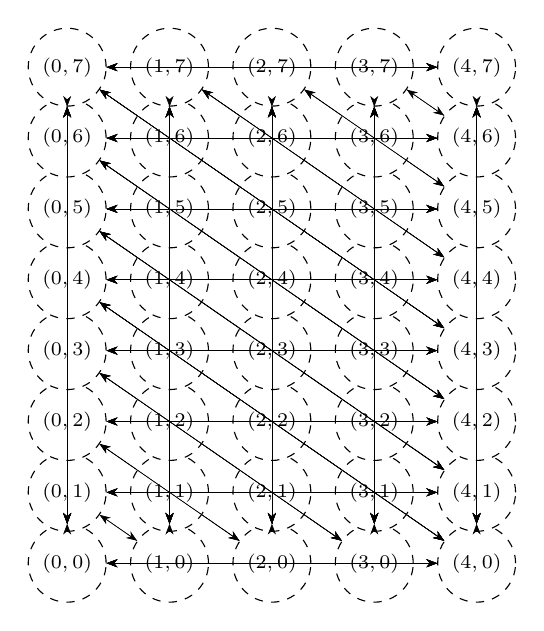
\begin{tikzpicture}[x=1.3cm,y=0.9cm,
    reachable/.style={circle,draw,fill=black!35,
                      minimum size=7mm,font=\scriptsize,thick},
    unreachable/.style={circle,draw,fill=white,
                        minimum size=7mm,font=\scriptsize,dashed,thin},
    >=Stealth,very thin]

% -----------------------------------------------------------
%  Reachable states (computed by BFS from (0,0))
% -----------------------------------------------------------
\def\reachableStates{
(0,0),(0,1),(0,2),(0,3),(0,4),(0,5),(0,6),(0,7),
(1,0),(1,7),
(2,0),(2,7),
(3,0),(3,7),
(4,0),(4,1),(4,2),(4,3),(4,4),(4,5),(4,6),(4,7)
}

% -----------------------------------------------------------
%  Draw all 40 nodes in a 5 × 8 grid, shading reachable ones
% -----------------------------------------------------------
\foreach \x in {0,...,4} {
    \foreach \y in {0,...,7} {

        % Test whether (x,y) is reachable
        \def\found{0}
        \foreach \p in \reachableStates {
           \ifx\p(\x,\y)\def\found{1}\fi
        }

        % Place node
        \ifnum\found=1
            \node[reachable]   (N\x\y) at (\x,\y) {$ (\x,\y) $};
        \else
            \node[unreachable] (N\x\y) at (\x,\y) {$ (\x,\y) $};
        \fi
    }
}

% -----------------------------------------------------------
%  Helper: draw arrow only if target is inside bounds
% -----------------------------------------------------------
\newcommand{\drawIfValid}[4]{%
   \ifnum #3>-1
   \ifnum #4>-1
   \ifnum #3<5
   \ifnum #4<8
       \draw[->] (N#1#2) -- (N#3#4);
   \fi\fi\fi\fi
}

% -----------------------------------------------------------
%  Generate all legal transitions directly from rules
% -----------------------------------------------------------
\foreach \x in {0,...,4} {
\foreach \y in {0,...,7} {

    % 1. Fill 4L
    \ifnum\x<4
       \drawIfValid{\x}{\y}{4}{\y}
    \fi

    % 2. Fill 7L
    \ifnum\y<7
       \drawIfValid{\x}{\y}{\x}{7}
    \fi

    % 3. Empty 4L
    \ifnum\x>0
       \drawIfValid{\x}{\y}{0}{\y}
    \fi

    % 4. Empty 7L
    \ifnum\y>0
       \drawIfValid{\x}{\y}{\x}{0}
    \fi

    % 5. Pour 4→7
    \pgfmathtruncatemacro{\t}{min(\x, 7-\y)}
    \ifnum\t>0
        \pgfmathtruncatemacro{\nx}{\x-\t}
        \pgfmathtruncatemacro{\ny}{\y+\t}
        \drawIfValid{\x}{\y}{\nx}{\ny}
    \fi

    % 6. Pour 7→4
    \pgfmathtruncatemacro{\u}{min(\y, 4-\x)}
    \ifnum\u>0
        \pgfmathtruncatemacro{\nx}{\x+\u}
        \pgfmathtruncatemacro{\ny}{\y-\u}
        \drawIfValid{\x}{\y}{\nx}{\ny}
    \fi

}}
\end{tikzpicture}
\end{center}
\caption{And here is the full reachability graph of 40 states.}
\end{figure}


\end{document}
